\chapter{TREVR Implementation In ChaNGa}
\label{sec:ChaNGa}
In this section we will give an overview of the Charm++ framework as well as the ChaNGa code that is built upon an extended version of the Charm++ framework. We discuss the methods used to develop the radiative transfer code and some of the challenges faced during implementation.

\section{Charm++}
Charm++ is a framework built upon the C++ language designed for applications in MIMD (Multiple Instruction, Multiple Data) parallel codes. Charm++ was designed to significantly reduce the quantity of coding work required when attempting to run parallel codes on multiple computer systems. This usually requires bespoke codes for every system in order to take into account memory type (i.e shared or distributed), message passing method and other system specific details \citep{Charm1}. This resulted in a large amount of developer time being spent on machine specific code rather than science related code. Through the use of the Chare class and object described in section \ref{sec:chare}, these issues are resolved via a runtime support system, hidden from the developer \citep{Charm2}.

Charm++ has several goals in its design: portability, where the same code can be run on all MIMD systems without modification; dynamic load balancing, where irregular parallel computations are handled so as to reduce core idle time; and latency tolerance, where requests for remote data do not force the core to idle while local work can still be performed \citep{Charm1}. Dynamic load balancing is performed through the use of Chare objects and latency tolerance through the use of a non-blocking message passing system. These are discussed in detail below.

Charm++ has been shown to scale excellently with large numbers of cores, as shown by the NAMD molecular dynamics code that showed speedup of 1599 times single core speeds when running on 2250 cores \citep{NAMD} although this simulation did not use the chare class, instead opting for custom Charm++ code. As molecular dynamics only has of order 100,000 computational elements (e.g. atoms in a protein), being able to divide work efficiently is a major achievement.

\subsection{The Chare Class}
\label{sec:chare}
The core component of a Charm++ program is the Chare class. The following outline of Charm++ and chares follows \citet{Charm2} and the Charm++ manual. Chares are concurrent objects that contain private data and a series of entry points, acting as the functions for the class. Each entry point takes a single input, a pointer to a message containing all data relevant to that function, and has no return value. As the Chare class is designed to avoid blocking remote access, it cannot contain public members. Chares can be distributed among all available cores and each core can hold multiple Chares. At any one time, a serial core only runs one Chare and that Chare only runs one entry function. This means that so long as the entry functions are written in such a way that they only modify local data, it is unlikely that race conditions will occur. Each Chare is given a handle unique across all processors that acts as its identifier for message passing which is handled by the run-time system for Charm++ rather than explicitly by the user.

A subclass of Chares, known as Branched Chares, have a branch on all processors. These are identified by a unique handler and share a similar definition syntax to standard Chares, with the addition of ``branched" at the start of their type definition. Once a Branched Chare has been created, usually by the main Chare, it is possible to call an entry function on all branches of that Chare simultaneously, allowing for simple control of all processes from a single command. Similarly, entry functions can be ran on an individual Chare by either calling them from within the Chare itself or by referencing its handle.

For every Charm++ program, there must be exactly one instance of the Chare type ``Main", executed on a single core. This begins the execution process and is often used to initialize shared variables and create new Chares. 

\subsection{Message Passing}

Message objects are utilized in Charm++ to allow for effective communication between chares and function scheduling while increasing code visibility to developers, aiding understanding and reducing complexity. These messages encapsulate all of the parameters to be sent to an entry method and thus different entry method calls can require different message types that can be created to hold any required data. This allows for developers to transfer data, including complex data structures, between chares without having to interact directly with message passing code.

Messages are stored when received by a core, requiring explicit deletion. This creates the risk of memory leaks as a result of poor programming practices but allows for messages to be acted upon in any order once received. When a message is created the programmer assigns a priority where lower values denote higher priorities by default. This is of particular use during tree walks as it allows us to prioritize messages returning data from remote walk data requests over local walk function calls, ensuring that the data is acted upon as received and freeing the memory required to store the message for further use. If multiple received messages have identical priority, they are computed in first-in-first-out order. 

\section{ChaNGa}
\label{sec:ChaNGa}
ChaNGa (CHArm N-body GrAvity solver) is an N-Body SPH and gravity solver adapted from GASOLINE. It was developed by the N-Body Shop research group at the University of Washington in collaboration with the University of Illinois Parallel Programming Laboratory to overcome the scaling issues encountered by GASOLINE on more modern machines whose processor counts are in the thousands \citep{ChaNGa1}. It is designed as an extension of the University of Illinois Charm++ framework. Specific extensions to basic Charm++ for ChaNGa include load balancing for adaptive timestepping. The core scientific modules are directly comparable to those of GASOLINE, with near identical methodology for SPH and cooling.

Like GASOLINE, ChaNGa uses a binary tree to split the simulation space but ChaNGa always splits cells in X-Y-Z order, effectively replicating an oct-tree every 3 levels. This allows Oct-tree-based methods for work distribution to be utilized \citep{ChaNGa1}. The tree is split into ``tree pieces", Chare objects (see section \ref{sec:chare}) that are distributed among the cores in use. By default there are 8 tree pieces created per core, each with a subset of the full tree. Each typically includes all the parent node information as well as all particles inside all nodes owned by the treepiece. All other particles must be requested as cached copies of the originals that are owned by other tree pieces. These other tree pieces can be both local (i.e. stored on the same processor) or remote (stored on another processor). 
\\
\\
\\
ChaNGa, again like GASOLINE, is designed to utilize adaptive time-stepping that allows for high time resolution in regions with short dynamic timescales without causing a substantial increase in wall time due to having to compute all particles at this timescale. Performance evaluations have shown up to 3x speedup over single stepping algorithms on NCSA's Blue Waters system \citep{ChaNGa3}

ChaNGa includes a system for ``checkpointing" where the entire state of the system is dumped to file. These checkpoints allow for the code to be restarted in cases such as hardware failure while ensuring no change to the output of the system. This is of particular importance when the data is highly sensitive to small changes in the system state, such as is the case in astrophysical simulations.

While regular checkpointing is recommended, the high cost of writing such a large quantity of data to storage requires a balance to be found between the possible data recovery gains and the cost in time.
    
\subsection{Space Filling Curves}

GASOLINE was developed to distribute data by splitting the data into a balanced binary tree, assigning the data on each leaf node to a core. This often led to the tree being split into long, thin slices and required a large amount of overhead, particularly when using more than 8 cores. This limited the scaling of GASOLINE, suggesting a need for a new method when developing ChaNGa.

For algorithms such as neighbour finding in particle methods or particle tracing in radiation (see section \ref{sec:ppWalk}), where the input data is in close physical proximity to the datum being computed, the data can be sorted, in theory decreasing the amount of overhead. This can be done by mapping the positions of the data to a space filling curve, a function that is continuous in space and can be iteratively refined so as to match the resolution of the data. This results in a large portion of the computation for each node using local data, with only the boundary data requiring requests to be sent to remote nodes.


While ChaNGa was initially built to use the Morton space filling curve (SFC), it was later adapted to use the Peano-Hilbert SFC. This curve is theoretically more efficient due to the lack of the Morton curve's sharp jumps. This increases data locality, where particles with close physical proximity also have close key proximity. This is an advantage in most serial and parallel computation. This also adds to the complexity of the code when calculating the physical bounds of the particles assigned to each node. Unlike the Morton SFC the Peano-Hilbert SFC rotates the shape used to create its curve, creating a disconnect between the spatially defined children and the ordering of the child nodes given by the SFC. For example, this removes the guarantee that child 0 of the node is assigned the particles who's indices are numerically lower than those of child 1, as shown in figure \ref{fig:SFC}. In this figure, the green regions show the cells with lower key values while the yellow shows that of higher key values. The Morton SFC's left hand child, equivalent to child 0, always contains the lower set of keys, unlike the Peano-Hilbert SFC. Because of this, the Morton SFC was utilized when running with the radiation code over the Peano-Hilbert SFC that is the default for ChaNGa.

\begin{figure}[H]
    \centering
    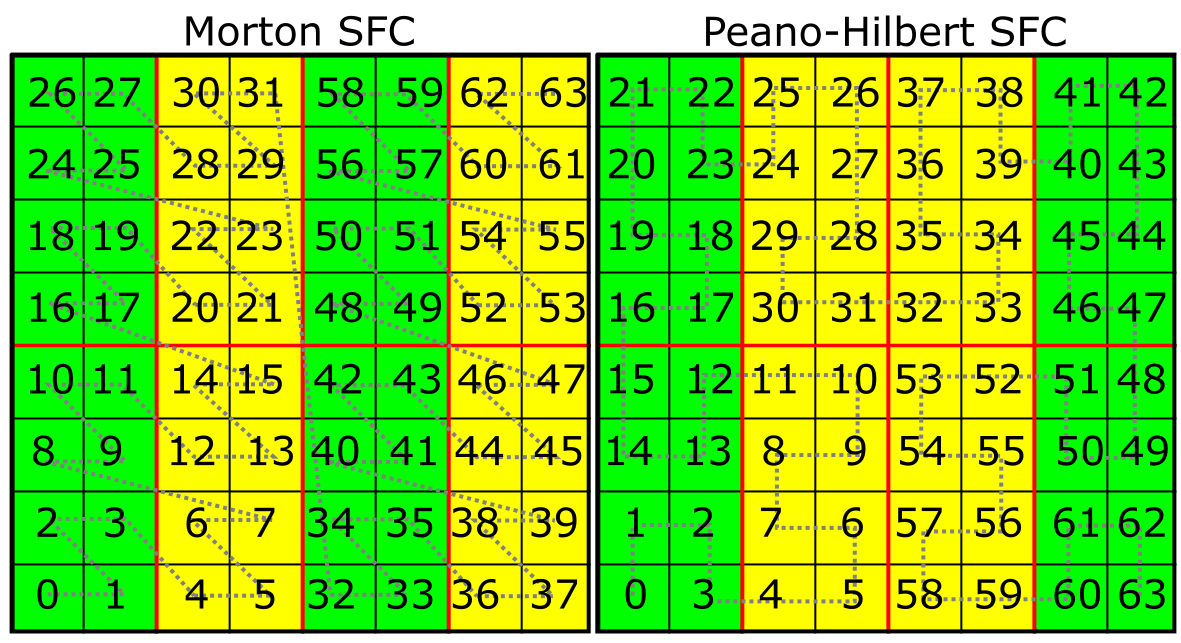
\includegraphics[width=\textwidth]{plots/CH3/SFCCompare.png}
    \caption{Diagram of Morton and Peano Hilbert space filling curves after 3 bisections (in the x, y and x axis respectively) 64}
    \label{fig:SFC}
\end{figure}

When the Morton SFC was replaced with the Peano-Hilbert SFC the bounds defining the node volume no longer consistently contained the particles assigned to the node. As a part of the tree build, the bounds are recalculated so that they define the minimum volume that contains all particles in the node (for identical reasons to those discussed for sources in section \ref{sec:sourceRef}). This bug remained undetected until the development of the radiation code as no other component of the code requires the exact spatial dimensions of each node and thus suffered no errors as a result of this. 

\subsection{The Tree Build}

To begin, the particles are assigned a key based on their position using a space filling curve (SFC). This curve is a fractal that can be refined as required to match the resolution of the particles in the system. These keys are then used during the tree build, where the particle set is bisected along each axis in turn to create child nodes. By bisecting at the key value associated with the bisection point in the space filling curve, we can accurately allocate the particles without having to check their individual positions, reducing the computational cost. This process is repeated for each node until the number of particles in the child node is lower than a predefined value. These final nodes are labelled bucket nodes and for ChaNGa the cutoff particle count is 12 although this can be changed by modifying the ``nBucket" parameter specified in the input parameter file for a given run.

Once the bucket nodes have been created the process is reversed, now walking from the bucket to the root. First, the node properties such as centre of luminosity and total luminosity are calculated for all buckets and then these values are propagated up into the parent nodes. This is repeated until all nodes have their properties calculated from their child nodes resulting in a tree that can be walked from both top down and bottom up depending on what is required.

While a new tree is built for every physics solver of GASOLINE, ChaNGa only builds the tree once per timestep, before any physical quantities (e.g. density or forces) are estimated, and uses it for every part of that timestep. Early in the development of GASOLINE the tree build was only a small fraction of the computational cost. The addition of adaptive timesteps has greatly impacted this as a tree must be built for each physics solver even if only a few particles are active, resulting in a large percentage of the time being spent building trees. 

While only building the tree once reduces overhead, it lacks the flexibility of GASOLINE's method where variables calculated in previous sections of the code can be easily included in the tree. For ChaNGa, an additional tree build is required once the required variables, such as density which is calculated as a part of the SPH code, have been calculated. This is a key issue for radiation due to the importance of density in the absorption coefficient. Values from prior time-steps could be used, either directly or through extrapolation.

A key benefit of the combined tree build is the simplicity it adds to the development of new code components. While implementing the radiation code, all that was required to propagate the radiation properties through the tree once they had been defined was two function calls: one for adding a new particle to a bucket and another for combining two child nodes into the parent node. These could be stored alongside the rest of the radiation code, minimizing the amount of code bloat that can arise from multiple new components being added to the original tree build. It also means that any modifications to the tree build will have little impact on the radiation properties so long as the function calls remain in the correct locations.

\subsection{Issues when developing on ChaNGa}

Unfortunately, development on ChaNGa suffers from several issues. The documentation lacks details on the specifics of developing the code other than for minor changes such as the addition of new parameters. This leaves those working on the more detailed sections of the code such as the tree build and data management systems reliant on comments in the code itself. These comments are often non-existent or insufficient and much time was required to properly understand their function. This combined with poor adherence to a standard formatting style leads to a difficult development process. Much of the code has substantial variation in indenting styles (or no indentation at all), comment format and variable name styles. Recently, efforts have been made to define a standard style for all collaborators to adhere to. Special thanks must be given to Tom Quinn from the University of Washington for the substantial amount of support and advice when developing the radiative transfer code, without whom many of the issues encountered would have taken far longer to resolve.

\section{TREVR in ChaNGa}

Although the core concepts behind the implementation of TREVR in ChaNGa are identical to those in GASOLINE, there are some key differences in the structure and methodology of the two codes that required new approaches to be developed.

\subsection{Top Down vs Bottom Up Tree Walk}

During the development of the radiation code for Gasoline, it was decided that the preferred method for the tree walk was a Bottom-Up approach, where the tree walk starts at the leaf node of the particle being walked from and moves up the tree till it reaches the root node. A second walk could then begin from the leaf node containing the source particle to the root, terminating if it reaches a node also walked by the sink.

Discussions with the developer Rory Woods revealed that this decision was made due to how the walk would focus resolution at the areas around the sink and source, areas which are often of the most interest when performing the ray trace. When using a refinement criterion to decide if a cell should be opened, this no longer holds true and the bottom-up tree walk acts in a similar way to the top-down tree walk but generally walks more nodes than necessary. While in the initial version of TREVR the refinement was purely geometric, the newest version of TREVR (\citealt{grond}) uses an adaptivity criterion instead.

Due to the more complex dual-walk method required for the bottom-up tree walk, the top-down tree walk was selected for implementation in ChaNGa. This method walks to both the sink and source simultaneously, removing the need to check if the second walk has reached a shared node with the first walk. This also has the benefit that if the system passes the refinement criterion on a high level node (such as for sources with a single or tightly clustered sources, as discussed in the next section), the tree walk can be completed very rapidly. Unlike the GASOLINE method, this means that for low average optical depths the computational cost of the optically thick tree walk can be less than $\mathcal{O}(log(N))$.

\subsection{Developing the Source Walk}

To begin the radiative transfer process we set up the book-keeping variables that allow us to keep track of how many remote data requests have been sent out for each bucket as well as which buckets have had their local and remote walks completed. We then loop through all buckets, starting both the local and remote walk for each. To allow for remote messages to be acted upon, the loop is paused at a set number of buckets and the function re-queued in the scheduler. This allows for local work to be performed while waiting for the remote requests and reduces the time that each core spends idling.

During the walk each node is checked against the opening criterion (see section \ref{sec:sourceRef}) to see if it requires refinement. If no refinement is required, the properties calculated via upwards propagation from the bucket are used to calculate the contribution to the flux from the the combination of sources in that node. If the node must be refined further, either the children of that node are walked or, in the case of bucket nodes, the flux contribution from each component source is calculated. This is repeated until the flux contribution from the entire system is calculated.

While the flux on each particle in the bucket is calculated using the individual particle's position, we use the centre of mass of the bucket as the basis for the opening criterion and thus all particles in a bucket have the same sources. This reduces the number of walks required by a factor of up to the maximum number of particles per bucket while adding minimal error.

\subsection{Source Walk Refinement criterion}
\label{sec:sourceRef}
Like the gravity code, the radiation code uses an opening angle based refinement criterion. The maximum distance from the centre of luminosity to the edge of the cell, $b_{max}$, along with the minimum distance between the sink and the physical boundary of the cell, $r$, are used to limit its angular diameter, giving,
\begin{equation}
    \label{eqn:openingTheta}
    \theta = \frac{b_{max}}{r}.
\end{equation}
A node is opened when the value of $\theta$ exceeds a predefined opening angle $\theta_{open}$.

As combining sources affects the accuracy of the calculated flux due to changes in the value of $r$, a balance must be found between computational savings and accuracy. To do this, the number of nodes walked, a good indicator of computational cost, can be calculated for multiple opening angles and the results compared to those for a fully opened version of the same system. This is explored further in section \ref{sec:bangForBuck}.

ChaNGa includes a collection of geometric intersection algorithms and it is thus easier to write equation \ref{eqn:opening} in terms of $r_{open}$, where $r_{open}$ is the radius of a sphere centred on the sink. If the rectangle defining the volume contained by a node intersects with this sphere, that node must be refined,
\begin{equation}
    \label{eqn:opening}
    r_{open} = \frac{b_{max}}{\theta_{open}}.
\end{equation}
The refinement criterion test can now be performed by creating a sphere of radius of $r_{open}$ and using the intersection algorithms to check if the sphere intersects the bounding cell of a node, as shown in figure \ref{fig:opening}.

\begin{figure}[H]
    \centering
    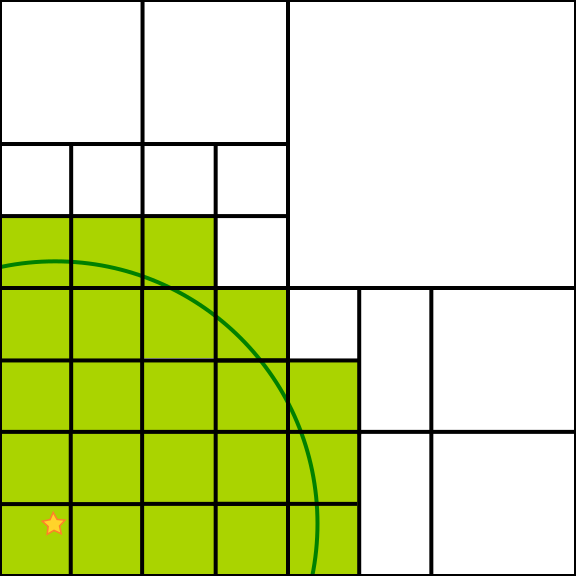
\includegraphics[width=0.9\textwidth]{plots/CH3/openingCritereon.png}
    \caption{Diagram of opening criterion for the source walk. All nodes that intersect the sphere of radius $r_{open}$, shown in green, are refined.}
    \label{fig:opening}
\end{figure}

Unlike gravity, where all particles inside a node contribute to its mass and thus must be considered, the only particles that contribute to the flux are sources, similar to how only SPH particles are considered during the fluid code. Because of this, a cell containing only the source locations can be considered when calculating the value of $b_{max}$. For a system with a single source, this means that the root node can accurately describe the entire system and thus the computational cost of the tree walk can be drastically reduced. In astrophysics, sources are often grouped together (star clusters, galaxies, etc) and thus this change should allow for less walking required in most applications. An example of this is shown in figure \ref{fig:sourceBoxes}.

\begin{figure}[H]
    \centering
    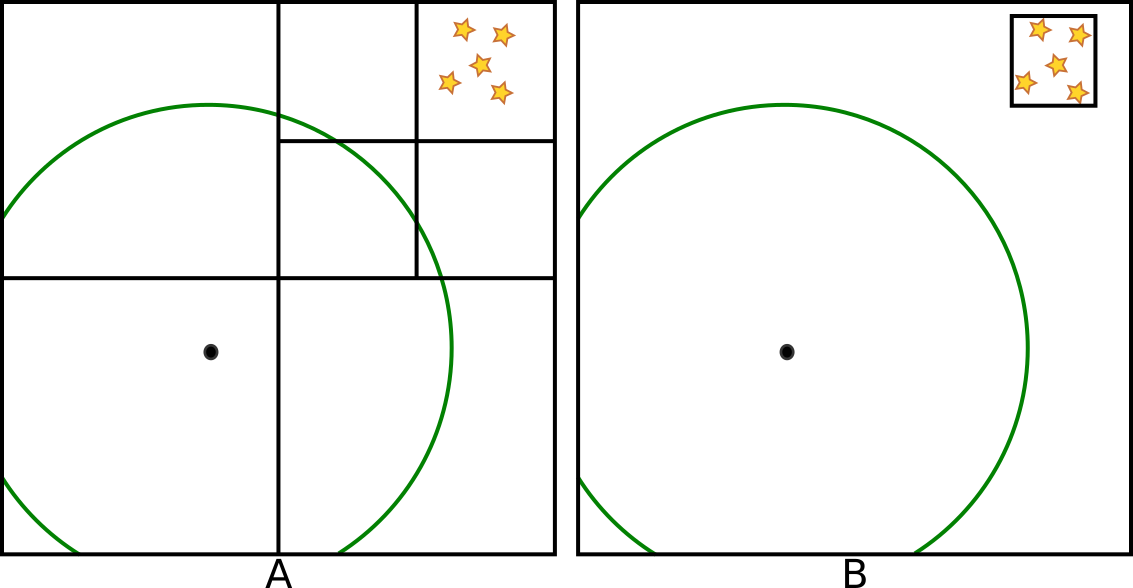
\includegraphics[width=\textwidth]{plots/CH3/sourceBox.png}
    \caption{Diagram of the effect of reducing the node's bounds so that they define the minimum volume that contains the node's source particles. A must refine to the 5th level in the tree whereas B can use the root node.}
    \label{fig:sourceBoxes}
\end{figure}

This is performed by utilizing code similar to that used for the pre-existing bounding boxes used for gravitational forces that are bounded by the particle positions in the node. To build a bounding box only containing the sources, first an empty box with zero volume is created and each source in the node is added through the use of the ``grow" function in the OrientedBox class used to define the node bounds. This updates the limits of the bounding box so that they contain all source particles in the node in the smallest possible volume.

\section{The Optically Thick Tree Walk}

\subsection{Developing the Optically Thick Tree Walk}

Instead of immediately calculating the flux contribution once a source has been located we store the source's position and total luminosity in an array for later use. As the source walk is run on the bucket rather than per particle, we only require one list of sources for all particles in a single bucket, reducing data usage. This results in a complete list of all sources for all sinks in the system once the source walk is complete. While this requires a large amount of data to be stored it has the benefit of allowing us to estimate the total flux on a sink before starting the optically thick walk. The uses of this are discussed in section \ref{sec:complexsources}.

The particles are walked one source at a time, with all sources for all particles in a bucket run before the next bucket is started. At the start of the walk, the optically thin flux is calculated for the sink-source pair being walked and stored in a placeholder variable on the sink. Once a walk is completed the sink particle being walked checks if any sources remain and if so begins the next walk.

During the walk, each node is checked for refinement, where nodes whose averaged absorption parameters are a poor estimate for the true optical depth through the node are refined (see section \ref{sec:thickRefine}). Once a node is selected, the length of the ray segment through that node and the node's absorption parameters are used to calculate the contribution to the optical depth. Once the full ray has been traced, the calculated optical depth is combined with the previously calculated optically thin flux to give the final flux via equation \ref{eqn:fluxThick}

\subsection{Calculating Optical Depths}
During the tree build, each bucket in the tree has all of its radiation properties calculated from its component particles. For the absorption coefficient, this was done originally through the method of summing each particle's product of mass and opacity and dividing by the total cell volume as shown in equation \ref{eqn:calcAbsCoeff} \citep{rory},
\begin{equation}
    \alpha_{bucket} = \frac{1}{N_{abs}}\sum_i{\frac{\kappa_i m_i}{V_{bucket}}},
    \label{eqn:calcAbsCoeff}
\end{equation}
where $V_{bucket}$ is the volume of the bucket, $N_{abs}$ is the number of absorbers in the bucket and $\kappa_i$ and $m_i$ are the absorber's opacities and masses respectively.

Unfortunately, this is susceptible to noise due to variations in particle counts per cell, especially if the number of particles in the cell is low . Solutions to this issue involve using a smoothed density estimate such as that estimated on each particle for SPH. These can then be averaged within a bucket. 

This creates a second issue where, because SPH, gravity and radiation are computed at the same time, up-to-date density estimates are unavailable during the tree build. Solutions to this second issue include using densities from previous timesteps, rebuilding the tree once density has been calculated, and extrapolating densities using known values. One such extrapolation method is to use the previous timestep's densities and the divergence of the particle velocities to give,
\begin{equation}
    \rho_i = \rho_{i-1} + \frac{d\rho}{dt}dt = \rho_{i-1} + \rho_{i-1} (-\bm{\bigtriangledown \cdot v} dt),
\end{equation}
where $\rho_i$ and $\rho_{i-1}$ are the current and previous timestep's densities respectively \citep{divV}.

Once the absorption coefficient for every bucket is calculated, the rest of the tree's absorption coefficients can be calculated by averaging those of each node's children.

During the tree walk, each node is checked to see if it intersects with the ray between the sink and the source and if so, the length of the segment contained within the node is computed. The node is then checked for refinement and if necessary the optical depth contribution for that node is calculated using the discrete form of equation \ref{eqn:tau}, shown below,
\begin{equation}
    \tau_{node} = \alpha_{node} s_{int},
\end{equation}

where $\alpha_{node}$ is the node's absorption coefficient (which includes the opacity term) and $s_{int}$ is the distance of the intersecting segment of the ray.

\subsection{Ray Trace Walk Refinement Criterion}
\label{sec:thickRefine}

As with the source walk, we need a method of deciding if a tree node is suitable for ray tracing or if it must be further refined. Just as the source walk's accuracy is decreased as sources are merged, the ray trace walk's accuracy is decreased when the absorption coefficients are taken from merged tree nodes.

Simply looking at the coefficients of the two children nodes is insufficient due to the ``smoothing" of the absorption coefficient as one moves up the tree. To resolve this issue, we instead create a best and worst case path through each node in all 3 dimensions. The best case path is set of buckets that gives the lowest optical depth through the node. For example, if looking for the best case path in the x direction, it would be the collection of buckets with the lowest absorption coefficients where no two buckets share the same position in the x axis. The positions in the y and z axis are unconstrained so that the buckets may not be continuous in space.

When two buckets are combined, the parent node stores the the greatest absorption coefficient or the averaged absorption coefficients of each child for each dimension depending on which dimension is being merged. (E.g. when merging two cells split along the x axis, the maximum in the x direction is the average of the two bucket's maximum absorption coefficients and the maxima for the other two directions are the greatest of the two absorption coefficients. Likewise for the minimum). This is then repeated on higher level nodes, with either the maximum/minimum or average of the maxima/minima absorption coefficients propagated, resulting in two values that represent the paths through the node with the thinnest and thickest optical depths. This path does not have to be physically possible for a ray to cross (i.e. the nodes used to create it do not have to be continuous in space) but it still provides as an effective bound for the theoretical error in each node. We must also take into account the length of the segment intersecting the node being walked. This prevents excessive refinement in the case of a small segment passing through a region with high variance in its absorption coefficient. While the percentage error for that segment may be large, the segment's overall contribution to the ray remains small enough that the total error is limited. This also allows us to use a single value for the opening criterion that will work for the entire ray trace.

To perform the refinement test, the difference in minimum and maximum absorption coefficient for all cardinal directions is multiplied by the segment length to give a theoretical maximum error in $\tau$, as shown in equation \ref{eqn:thickRefinement},
\begin{equation}
    \delta\tau = l_{seg}(\alpha_{max} - \alpha_{min}),
    \label{eqn:thickRefinement}
\end{equation}
where $\delta\tau$ is the error in $\tau$, $l_{seg}$ is the segment length and $\alpha_{min}$ and $\alpha_{max}$ are the minimum and maximum $\tau_{refine}$ through the node. If $\epsilon_\tau$ exceeds the refinement parameter the node is opened and the children walked. To avoid self absorption, we also refine all nodes whose bounds lie or partially lie within the smoothing length of the sink being walked. This refinement creates an approximation of a sphere inside which the ray tracing moves from particle-node absorption to particle-particle absorption.

\subsection{Particle Level Ray Tracing}
\label{sec:ppWalk}
While node-level calculations of the optical depth are simple, only requiring the appropriate node to be selected via the opening criterion, refinement to the particle level requires more consideration. To correctly resolve ionization fronts (such as those seen in Str{\"o}mgren sphere tests) the ray must be traced through all particles in close proximity to the sink being analyzed. This prevents the sharp jump in opacity at the ionization front from being smoothed out by the averaging of properties during the tree build. This portion of the computation is referred to as Particle-Particle (PP) absorption. The method used for this was adapted from that used in the GASOLINE implementation of this code \citep{rory}.

To begin, the gas particles needs to be converted into a form that can be ray traced. To do this, we flatten the particle into a 2d disk in the plane perpendicular to the ray, with radius equal to its smoothing length, h (as calculated in the SPH code). We then need to calculate the minimum distance between the ray and the absorbing particle's position. As the ray is defined by the line between the sink position and source position, this distance can be calculated using the following equation,
\begin{equation}
d = \sqrt{||\bm{x}_0 - \bm{x}_2||^2 - \frac{((\bm{x}_0 - \bm{x}_2) \cdot (\bm{x}_1 - \bm{x}_2))^2} {||\bm{x}_1 - \bm{x}_2||^2}},
\end{equation}
where ${\bm{x}_0}$ is the particle location and ${\bm{x}_1}$ and ${\bm{x}_2}$ are the sink and source particle locations respectively.

Once we have this distance, we can calculate the optical depth contribution by passing the distance and smoothing length of the particle to an integrated smoothing kernel, giving us a contribution to $\tau$ of,
\begin{equation}
\tau_i = \kappa_i m_i \int{W \bigg(\frac{d_i}{h_i}\bigg)}ds,
\end{equation}
where $\kappa_i$, $m_i$ and $h_i$ are the absorber's opacity, mass and SPH smoothing length, $W(x)$ is the SPH smoothing kernel function and $ds$ is the segment of the ray intersecting the absorbing particle.

This smoothing kernel, shown in figure \ref{smoothingKernel}, represents the radial distribution of the absorbing mass over a sphere whose radius is equal to twice the smoothing length. Integrating this gives the effective density of a path through the sphere perpendicular to the radial direction. 
\begin{figure}[H]
    \centering
    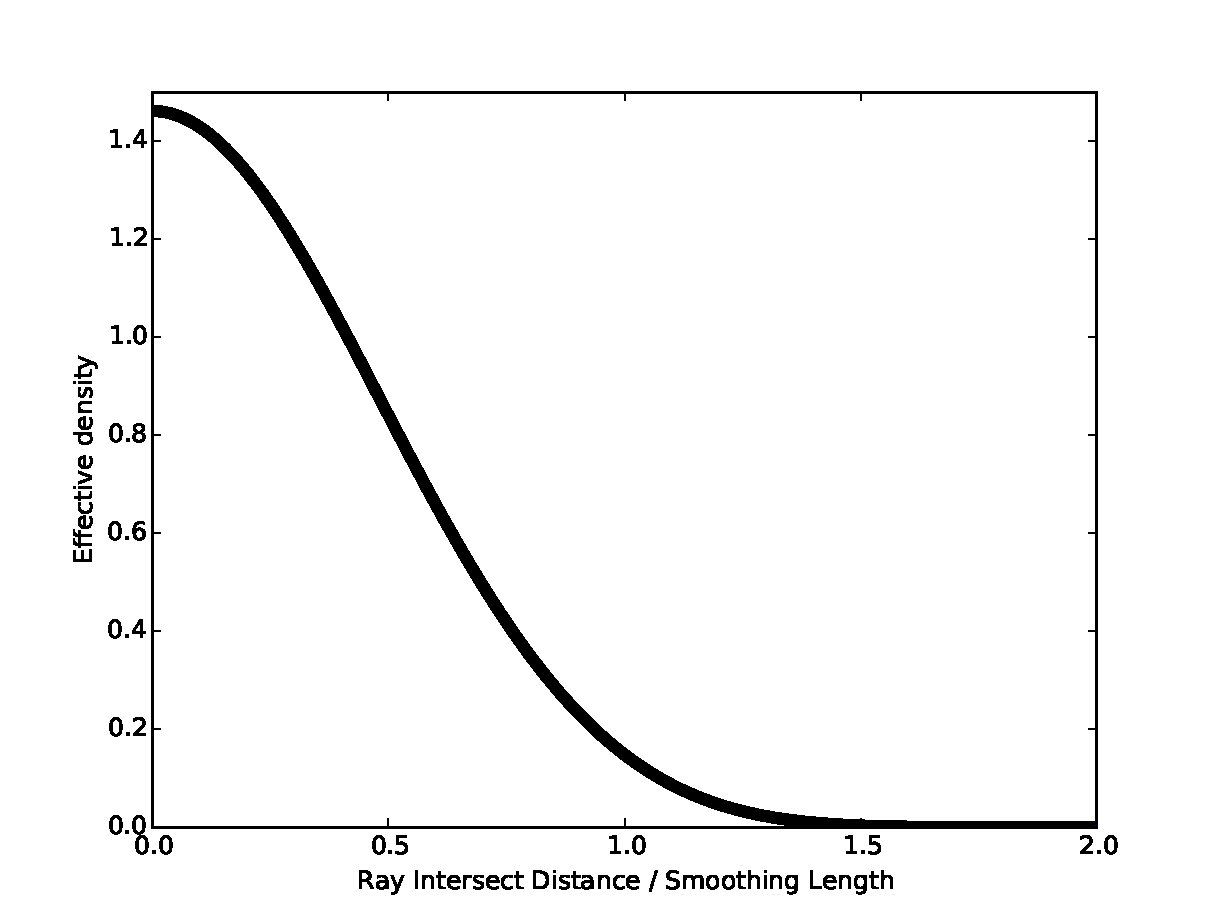
\includegraphics[width=0.85\textwidth]{plots/CH3/kernelPlot.pdf}
    \caption{Effective density of the M4 Cubic Spline smoothing kernel against radial distance from the particle}
    \label{smoothingKernel}
\end{figure}

While particle level tracing is only performed on particles within a chosen radius, in this case set as the SPH smoothing length of the source particle, efforts must be made to ensure that all particles who's smoothed mass fall within this radius are included. This may include particles in nearby cells that do not intersect with the ray even though some of their component particles do intersect due to the extra width generated by their smoothing lengths. For this, we initially refine all nodes within $h_{source} + h_{max, node}$ of the source, where $h_{max, node}$ is the maximum SPH smoothing length within the node. All particles within this distance are then sampled as normal.

Checks must be made to ensure that the particle does not contribute to its own optical depth as this can lead to substantially reduced flux values, particularly in matter with high optical depths. One other issue that must be prevented is where particles in close proximity all contribute each others optical depths due to overlapping smoothed mass regions, as shown in figure \ref{fig:ppOverlap}. This is the equivalent to two objects both being in front of each other simultaneously, a physical impossibility. To prevent this, all particles with a radial distance between themselves and the source greater than that of the sink particle being computed are ignored during the ray trace. This allows for optimization by ordering all particles in the node by ascending radial distance before performing the P-P calculation and ending the calculation at the first particle whose radial distance is too great. 

\begin{figure}[H]
    \centering
    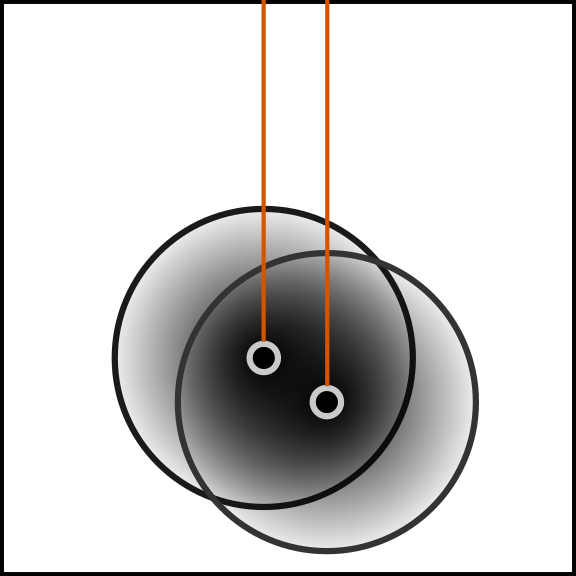
\includegraphics[width=\textwidth]{plots/CH3/ppOverlap.png}
    \caption{An example of two particles each contributing to the other's optical depth due their rays intersecting each others smoothed mass region.}
    \label{fig:ppOverlap}
\end{figure}
